\section{Desarrollo}
\subsection{Estructura del proyecto}

Uno de los puntos buenos que tiene este \textit{framework} es
poseer una estructura de directorios bien conocida y definida,
por ello será fácil navegar por ella incluso para nuevos
desarrolladores que se incorporasen al proyecto.

\medskip
Los principales directorios son los siguientes:

\begin{itemize}
    \item /src/app/: ficheros de configuración de la aplicación.
    \item /src/assets/: ficheros multimedia y recursos estáticos.
    \item /src/enviroments/: ficheros de configuración para los
    distintos entornos (desarrollo o producción)
    \item /src/pages/: directorio donde van ubicados los directorios
    de cada pandalla o componente de la aplicación.
    \item /src/pages/page1/: ficheros referentes a una pantalla en
    concreto en el van el HTML, TS, SCSS (si fuese necesario)
    \item /src/providers/: ficheros de acceso a los datos.
    \item /src/theme/: fichero de estilo genérico en el cual
    se basa la aplicación.
\end{itemize}

\medskip
Como se ha indicado en anteriormente en el proyecto existen distintos
tipos de ficheros según su objetivo a cumplir, obtener información,
dar formato a los datos para mostrar los mismos, configuración, etc.
A continuación se pasará a mostrar algunos extractos que se han
considerado relevantes.

\begin{figure}
    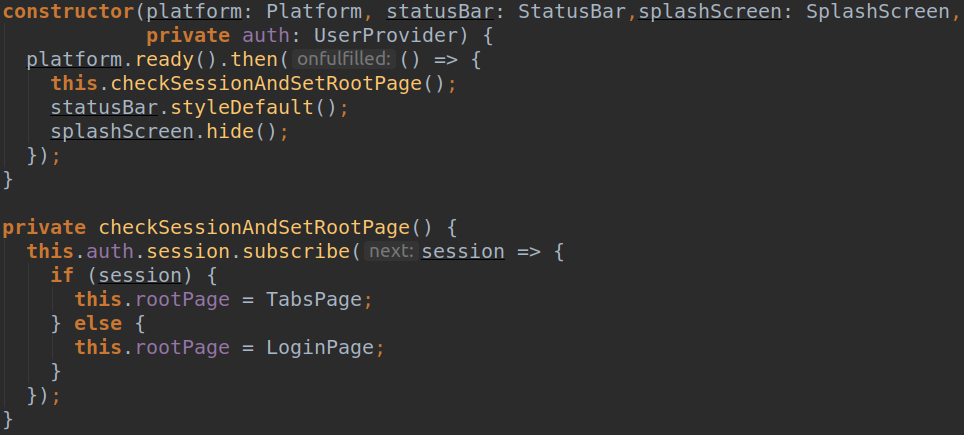
\includegraphics[width=\linewidth]{./images/code/app-components-ts.png}
    \caption{Fichero app.components.ts, control de sesión.}
    \label{app.components.ts}
\end{figure}

\medskip
En la \textbf{figura \ref{app.components.ts}} se puede ver como se gestiona
el control de sesiones, con ello la aplicación no permite el uso de ninguna
funcionalidad si el usuario no ha iniciado sesión. Como se muestra si este
no ha iniciado la sesión se le enviará a la página \textit{LoginPage} la cual
permite el inicio de sesión y da acceso al registro para el caso de usuarios
que no se han dado de alta en el sistema. Si en caso contrario si que existe
una sesión por parte del usuario a este se le enviará a la página principal
de la aplicación \textit{TabsPage} en la que se encuentran las distintas
ventanas disponibles separadas por una barra con pestañas.

\begin{figure}
    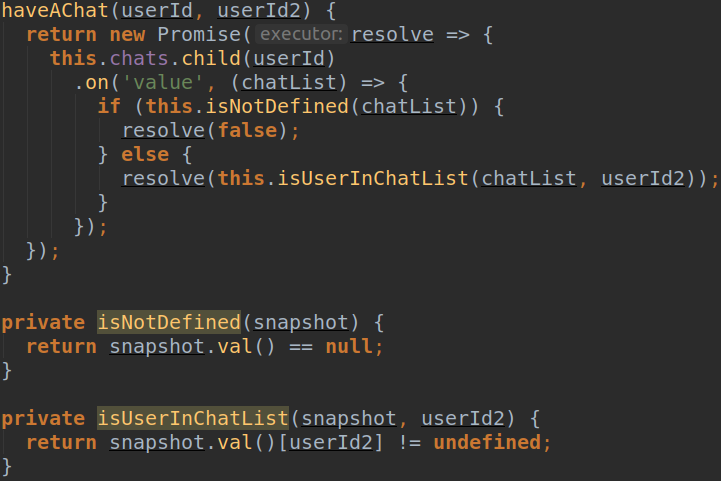
\includegraphics[width=\linewidth]{./images/code/chats-provider-haveAChar.png}
    \caption{Fichero chats.ts, función haveAChat.}
    \label{chats.ts.provider}
\end{figure}

\medskip
En esta \textbf{figura \ref{ejercicios}} se quiere mostrar la importancia que
tienen los nombres en las funciones y la importancia que se le ha dado a
estos durante todo el desarrollo. Se puede ver como con un simple vistazo
cual es el objetivo de esta función, saber si un usuario tiene un
chat abierto con otro. Una vez dentro de esta se puede casi leer como
si de una frase se tratase, "este chat tiene un hijo con este id de usuario
en la lista de chats" Si se continúa leyendo a partir de la línea cinco
obtenemos "si no está definido resolvemos que no tiene un chat y en
caso contrario comprobamos está el usuario en esta lista y lo transmitimos"
Es por los buenos nombres en las funciones, parámetros y el definir funciones
cortas lo que hace que este código sea legible y entendible sin tener
que realizar grandes esfuerzos. Estas son algunas de las reglas de código limpio\cite{clean-code}
que se han tratado de transmitir con este proyecto, a los desarrolladores
que posteriormente puedan leer este código. Reglas que se han considerado
de vital importancia pues si se quiere una aplicación longeva que sea fácilmente
sostenible y ampliable, esta tiene que ser en un primer momento, al menos,
entendible por los trabajadores que se tengan que enfrentar a ella.

Otra de las leyes o normas que se cumple es un efecto secundario de usar
buenos nombre, se trata de no usar comentarios. Al estar bien nombrados
los comentarios pierden valor, debido a que el propio nombre es explicativo
es por ello que no es necesario poner comentarios explicativos en el código.
Por último nombrar un principio más que se puede ver como se cumple en este
código, se trata del principio de responsabilidad única. El cual dice
que una función solo debe hacer una cosa, no debe llamarse tieneUnChat e
internamente comprueba si tiene un chat y asigna uno en caso de que no lo tenga
si fuera así estaría mintiendo con el nombre y se podría hacer un mal uso de este
o generar problemas porque tiene un comportamiento que no se espera.

\begin{figure}
    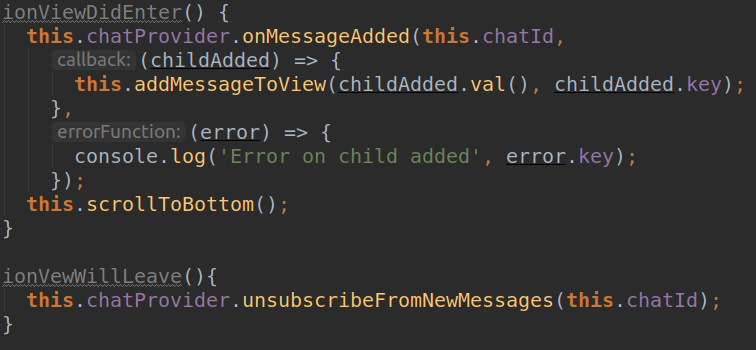
\includegraphics[width=\linewidth]{./images/code/view-chat-ts-onViewDidEnter.png}
    \caption{Fichero view-chat.ts, función onViewDidEnter.}
    \label{view-chat.ts}
\end{figure}
\medskip
Para mejorar la experiencia del usuario se ha tenido en cuenta en la carga
de datos usar las funciones que nos da ionic como son \textit{ionViewDidEnter}
y \textit{ionViewWillLeave} para cargar la información mientras la pantalla
se renderiza, de esta manera al no hacerlo en el momento que la pantalla
ya está mostrada el usuario no tendrá que esperar en una pantalla en blanco
a la llegada de estos pues los datos están siendo solicitados al servidor
en el momento que se empieza a preparar la pantalla para mostrarse. De igual
forma este no tendrá que esperar a que se cierre la conexión con la base de
datos para cerrar esta pantalla, en el momento que se comienza la "destrucción"
de la misma el sistema laza la desconexión de manera asíncrona.